%!TEX root =../../thesis-ex.tex

\section{Definition of Decision Making and Decision Support Systems}

In this thesis, we consider both user decision and decision making as their most general sense possible. Decision making is the activity for a user to interact with systems on her device, where the user have to choose from a set of options, and the selection is related to the users' personal benefit, e.g., money, security, or a significant amount of time. 

Under this definition, most activities for the user to interact with an information system (i.e., search engine or recommender system) are within the scope of decision making. For example, when a user needs to make selection for which paper to read next, or which movie to watch next, it may require a significant amount of time, therefore these activities should also be categorized as decisions. Interactive activities that we do not consider as decisions are tasks where the interactions are fixed and without much uncertainty, e.g., the how-to activities such as how to attach a photo to a Tweet. 

Similarly, we consider decision support systems a general concept. A decision support system is any system that provides information more than the original information and assist users reduce the uncertainty of decision making. As a result, any recommender system (e.g., people who bought this also bought) is a decision support system under our definition, because the suggested items allows users to observe similar items more efficiently which could potentially lead to a purchase decision. A question answering shopping agent is also a decision support system because it helps the users to reduce the uncertainty for a produce. Therefore, the decision support can be in two ways: first, the system initiate the decision support by actively providing information; second, the system support decisions on demand and provide the information specified by the user. 

\section{Motivation for Three Decision Making Problems Studied}
\label{ch1:sec3:overview}

Despite the work done by Google on knowledge support on mobile devices, there still exists many problems where such knowledge is not available on mobile results for bridging the gap, or the provided knowledge entry can be further optimized. In this thesis, we study knowledge support for the following three decision making challenges for mobile users. 

\textbf{Assisting Shopping Decision Making}. Users' shopping decisions often involve the need for them to understand and manage complicated product features, e.g., to purchase a computer, the user needs to know what brands she wants to purchase, her budget and what is the price distribution of the products, or even the relation between price and features, e.g., \emph{what is the minimum price I need to pay for a computer with 16GB ram?} Without knowing such knowledge, it is more challenging to issue a meaningful query. For example, the user may want to add to the query a brand name which she saw 10 products above the current position. With mobile screens, it can be more difficult to navigate that product. On the other hand, when completing the query, the query expansion results overrides the search results, making it more difficult to edit the query while viewing the products at the same time. 

\begin{figure}[h]
\centering
\subfloat[][Desktop showing search results and query suggestion at the same time]{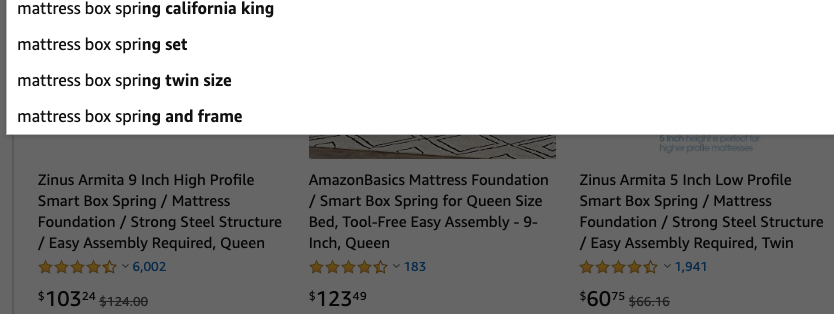
\includegraphics[width=.65\textwidth]{figure/chapter1/overview2}\label{ch1:fig2:overview2}}\hfill
\subfloat[][Mobile showing query suggestion only]{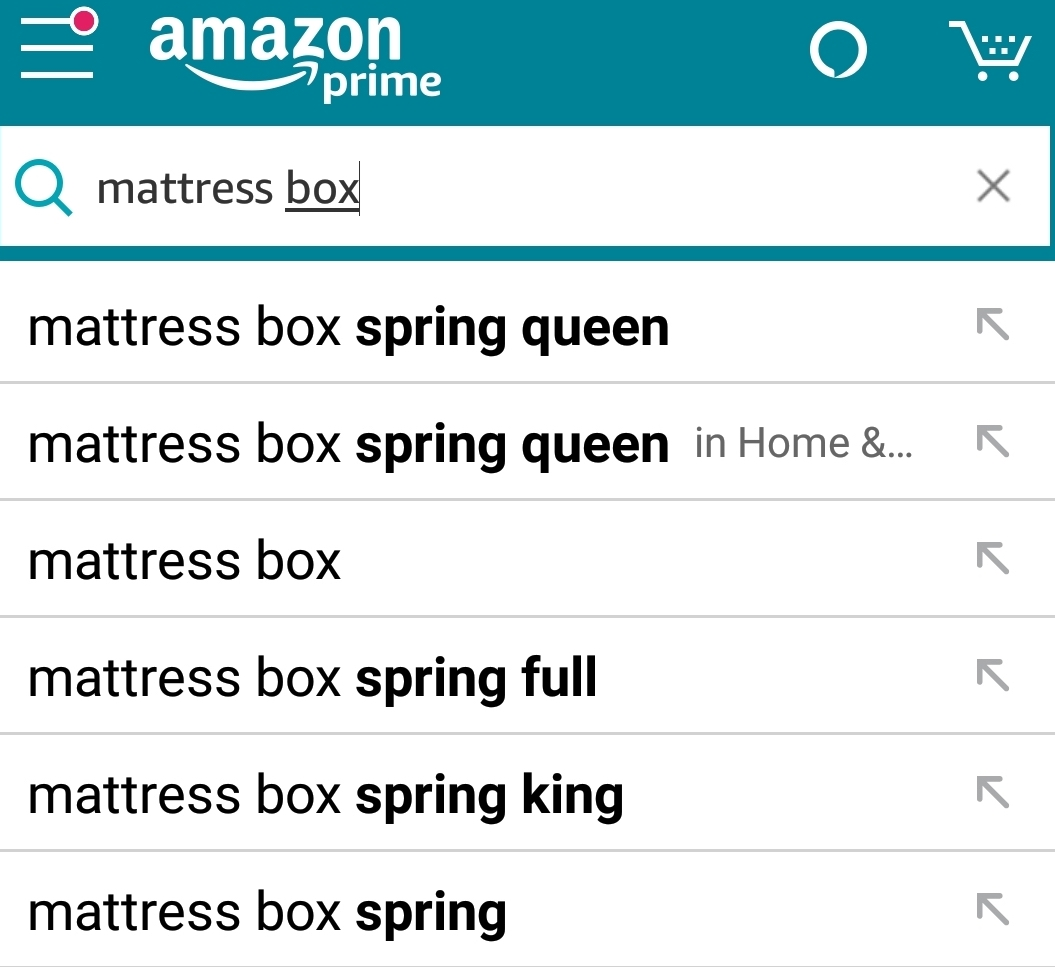
\includegraphics[width=.27\textwidth]{figure/chapter1/overview1}\label{ch1:fig2:overview1}}
\caption{The difference in query expansion interfaces on desktop and mobile: desktop displays the search results and query expansion at the same time; on the other hand, mobile query expansion page overrides the search results, therefore it is more difficult to add keywords to the query, e.g., \emph{zinus}}
\end{figure}

To support user navigation on mobile devices, e-Commerce apps often provides a faceted search system, which shows ranked lists of the meta data of products, e.g., brands, price distribution, screen sizes. By navigating the system, the user does not need to remember the features, but can directly click on the facet values to filter the results, e.g., \emph{brand = Dell}. 

Faceted search system makes navigation on mobile devices easier, however, by the time the study was conducted, an important component had not been optimized, which is the numerical facets of products. As discussed above, users often need to learn the price distribution of a product before making a salient decision. The numerical facets also helps users more conveniently navigate to the subset of products whose prices are within the ranges more relevant to users. By the time the study was conducted, however, a majority of numerical facets are predefined, so that the website shows the same price distribution for diamond ring and greeting cards. The same results offer no clue for price distribution of these products. Meanwhile, it also increases the difficulty for navigation. As a result, for the first problem, we study the problem of optimizing numerical facets for assisting shopping decision making. 

\textbf{Assisting Security Decision Making}. Mobile systems introduce a new decision making task for users: security decision making. Android permissions control the access for mobile applications to access users' private data resources, e.g., user location, contact list. In the earlier versions of Android, the permissions are requested during installation time (Figure~\ref{ch1:fig2:android1}), and users must accept those permissions before they can install the app. Meanwhile, the system does not support any explanation to be added to the interface in Figure~\ref{ch1:fig2:android1}, therefore the knowledge support for decision making was not possible by design. In Android 6.0 and later (Android Marshmallow), the permission system was replaced by a runtime model, where the permission requests can be postponed until it is used during runtime (Figure~\ref{ch1:fig2:android2}). This new design thus allows the knowledge support to appear by inserting a new layout before or after the permission request. The latest version of Android (Android Q) keeps the runtime permission but also allows the install time permission to be granted individually, so that users have more opportunities to make decisions. iOS has a similar permission requesting interface, but more conveniently, the developer can display the explanatory sentences right on the permission requesting page. 

\begin{figure}[h]
\centering
\subfloat[][Install-time Permission]{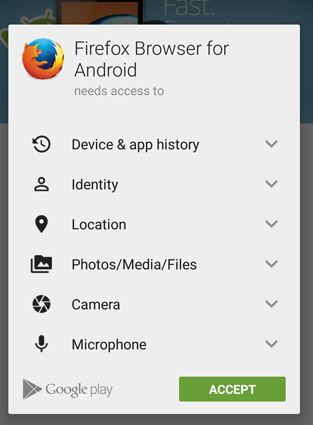
\includegraphics[width=.25\textwidth]{figure/chapter1/android1}\label{ch1:fig2:android1}} \hskip 40pt
\subfloat[][Android M (Runtime)]{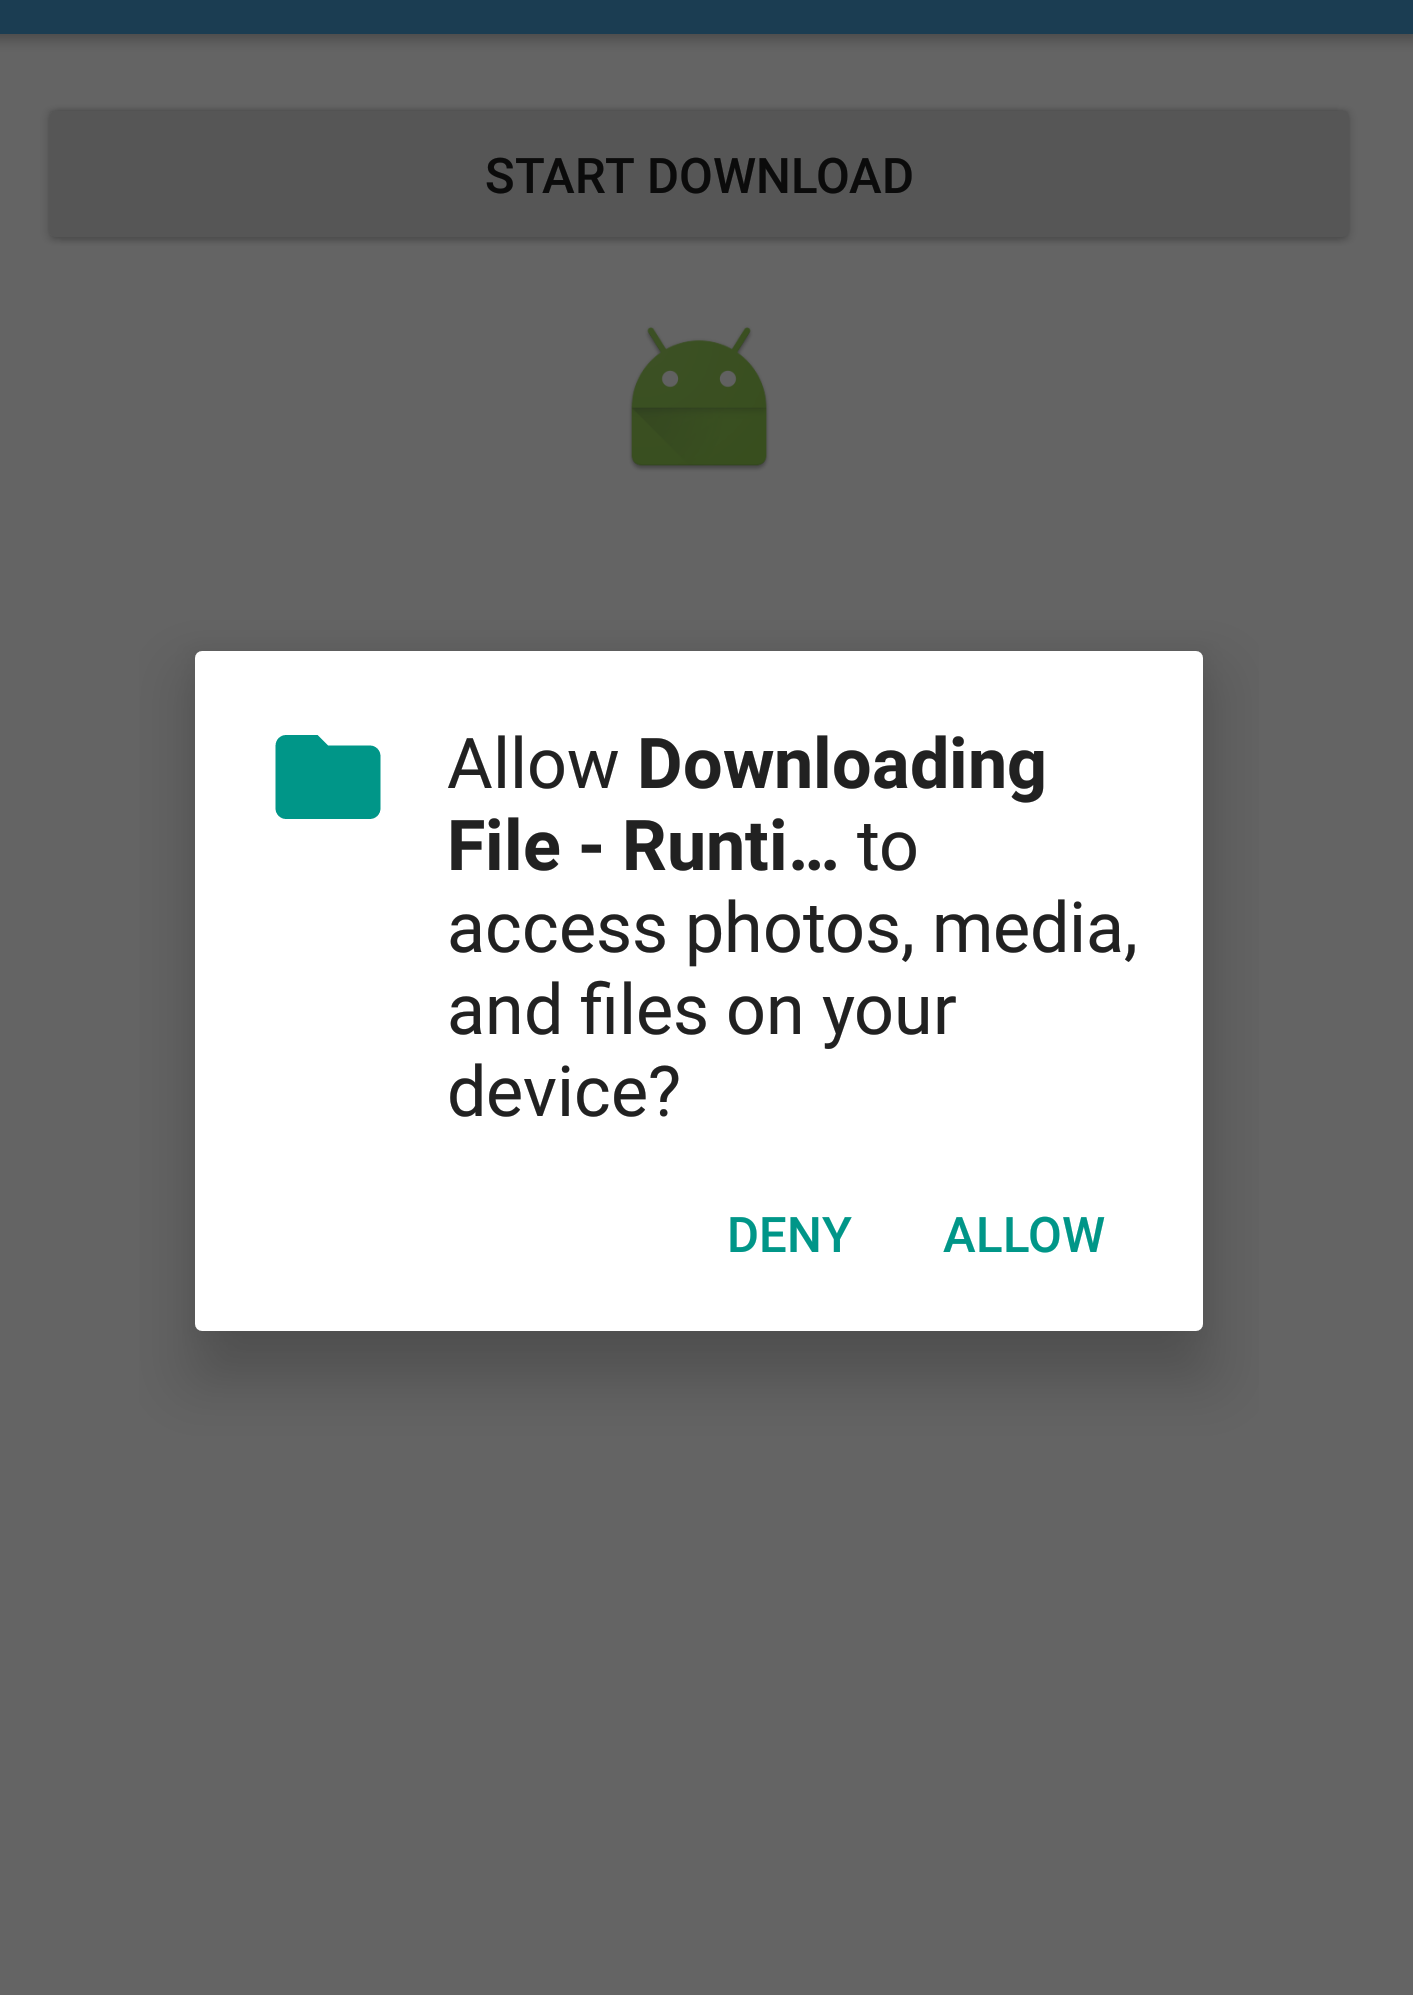
\includegraphics[width=.25\textwidth]{figure/chapter1/android2}\label{ch1:fig2:android2}} \hskip 40pt
\subfloat[][Android Q]{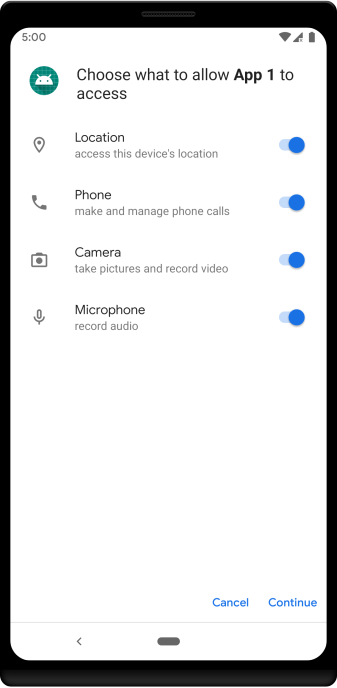
\includegraphics[width=.25\textwidth]{figure/chapter1/android3}\label{ch1:fig2:android3}}
\caption{The three Android permission models: install-time permission (all permissions are requested at install time); runtime-permission (permission can be delayed at the runtime); and the latest permission model (permissions can be requested at both the install time and runtime permission)}
\end{figure}

Although the newer permission models have allowed the applications to support knowledge to users for making security decisions, such changes do not guarantee that developers \emph{will} provide such knowledge. Indeed, we can always find news articles or forum posts complaining that Android permission purposes are confusing. As a result, we propose to study two problems: first, have Android apps provided sufficient knowledge supports for users' security decision making; second, if not enough knowledge are provided, how can we assist developers to improve the decision support. 

\textbf{Assisting Data Analytics for Business Decision Making}. A general strategy to support users' decision making, especially business decisions, is to support data analytics, including database queries. For example, the user may want to make a decision according to last years' sales record. On desktop/laptops, the decision making usually involves querying of a database. However, novel data analytics may not be familiar with SQL grammar. As a result, it would be convenient to support a natural language interface to assist the decision making. Figure~\ref{ch1:fig5:powerbi1} shows an example of such a natural language interface. When the user input the natural language question ``what is the breed of the dog named betty'', the system translates it into an SQL statement: \texttt{SELECT breed FROM dogs WHERE name = betty}, and displays the execution result. 

\begin{figure}[h]
\centering
\subfloat[][Conversational data analytics tool in Power BI (desktop)]{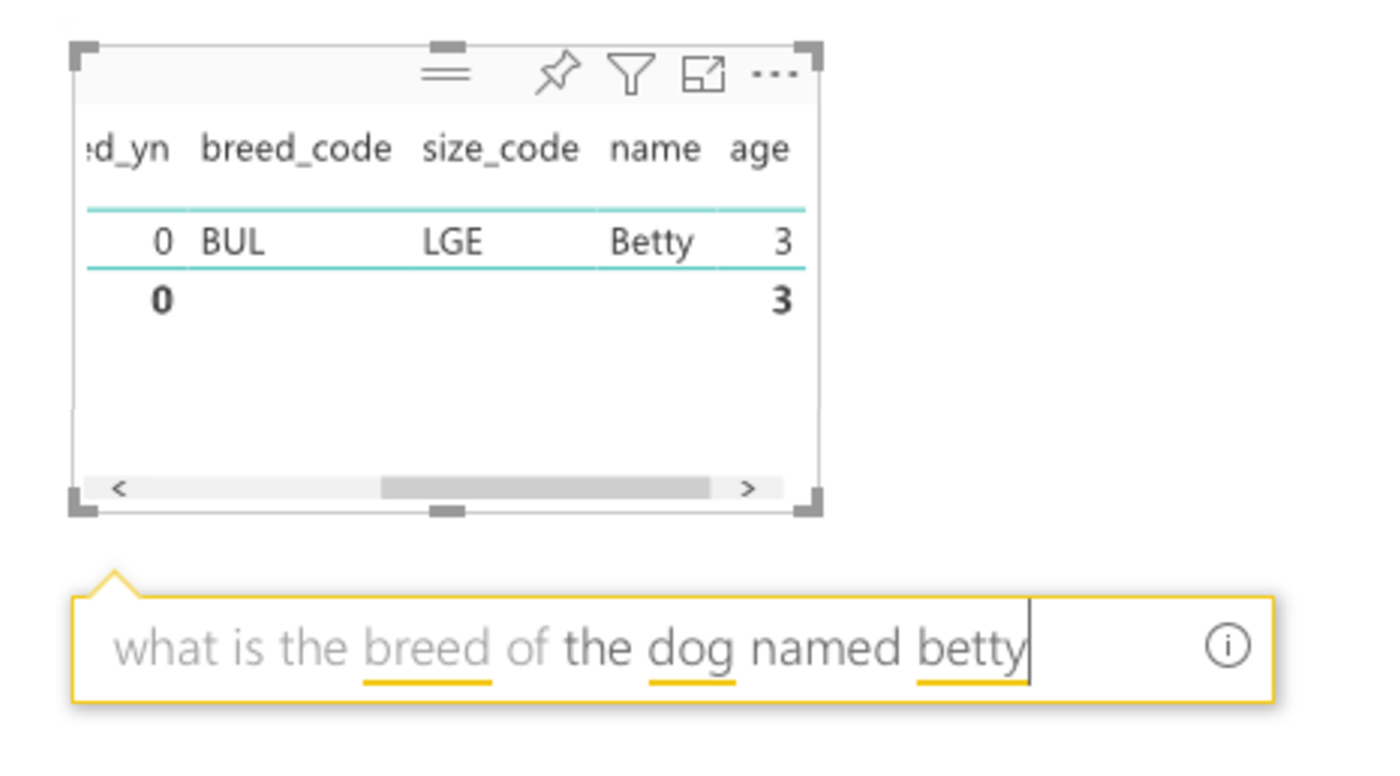
\includegraphics[width=.5\textwidth]{figure/chapter1/powerbi1_crop}\label{ch1:fig5:powerbi1}} \hskip 40pt
\subfloat[][Power BI iOS]{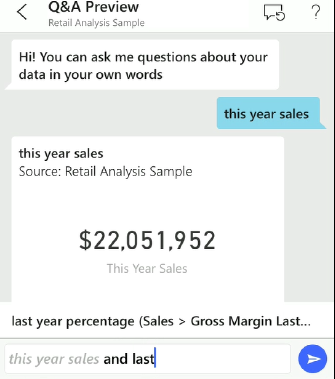
\includegraphics[width=.25\textwidth]{figure/chapter1/powerbi2}\label{ch1:fig5:powerbi2}} 
\caption{Microsoft Power BI interface (left) and the corresponding mobile application (right)}
\end{figure}

Mobile business intelligence is a new area (less than 10 years). However, surveys show that in 2017, 28\% percent of BI users stated that mobile BI was already in use in their company, with 23\% planned to be in use in the next 12 months and 22\% planned in the long term~\cite{mobilebi}. As of 2019, many mobile BI tools are in use. For example, Microsoft Power BI introduced the iOS application in 2015. Similar as the desktop version, the mobile applicaion also support the natural language interface feature (Figure~\ref{ch1:fig5:powerbi2}). 

To assist mobile users with business decision making, it thus is an important task to support natural language interface, i.e., translating the users' natural language question into SQL statement. Due to the aforementioned difficulty in mobile user interaction (i.e., small screen, difficulty researching information), it may be particularly difficult to write a correct SQL statement, therefore the support of natural language interface is particularly helpful. 

In these BI platforms, the NL2SQL must adapt to new database schemas provided by the user. As a result, the predictor must be able to generalize to new domains which has not been seen in the training data. The problem of cross-domain NL2SQL with complex query structure is still an active research area that has not been well solved. The problem of State-of-the-art approaches can achieve an accuracy of 65.5\%. As a result, we study the problem of translating natural language to SQL for cross-domain complex queries. 

\section{Organization of This Thesis}

The rest of this thesis is organized as follows. 

$\bullet$ \textbf{Chapter~\ref{ch2:shopping}: Assisting Shopping Decision Making with Numerical Faceted Search}. We study the problem of optimizing numerical facets to support users' shopping decision making on mobile devices. With a 2-month user query and click log on \url{www.walmart.com}, we develop a machine learning algorithm that suggests numerical ranges given a query. First, we propose an evaluation metric that evaluates the performance of a numerical range suggestion algorithm (Section~\ref{ch2:metric}). Based on the proposed metric, we propose three optimization algorithms by optimizing the metric directly (Section~\ref{ch2:dp}) and its upper bound (Section~\ref{ch2:percentage}). 

$\bullet$ \textbf{Chapter~\ref{ch3:runtime}: Empirical Study on Knowledge Support for Security Decision Making}. Before studying assisting users' mobile security decision making, we need to first empirically study whether existing applications have already provided sufficient explanations to support such decision making. Using sentence classification techniques, we creates a new dataset containing the explanation sentences by mobile applications. We propose five research questions to evaluate the sufficiency of explanations. Statistical significance tests show that generally, the decision support has not been sufficient compared with the suggestions by Android developers documentation. 

$\bullet$ \textbf{Chapter~\ref{ch4:clap}: Recommending Explanation to Assist Security Decision Making}. By identifying the deficiency in decision support, we propose to assist application developers to improve their existing explanations. By leveraging a large dataset containing the meta data of 1.45 million Playstore applications, we collect a large scale text corpus. By leveraging information retrieval techniques and unsupervised truth finding, our recommender system can suggest highly relevant sentences to the true purpose of the application. Qualitative evaluation shows the suggested sentences show three characteristics of interpretability. 

$\bullet$ \textbf{Chapter~\ref{ch5:nl2sql}: Assisting Business Decision Making with Natural Language to SQL Interface}. We study the problem of how to help mobile BI by supporting the natural language interface (NLI, or NL2SQL). We leverage a large complex cross-domain dataset named Spider to more closely simulate the scenario of mobile BI. By leveraging database values, we successfully matched database values that has been mentioned in the natural language question. We inject the matched database values to the existing state-of-the-art model on Spider, and observe 2.7\% improvement in the exact matching accuracy of output SQL statement. We further conduct an empirical study~\ref{ch5:sec:study} to explore potential ways for further improvement. 
